\chapter{Lead Titanate}
\label{chap:Materials}
\thispagestyle{empty}


%%%%%%%%%%%%%%%%%%%%%%%%%%%%%%%%%%%%%%%%%%%%%%%%%%%
%%%%%%%%%%%%%%%%%%%%%%%%%%%%%%%%%%%%%%%%%%%%%%%%%%%
%%%%%%%%%%%%%%%%%%%%%%%%%%%%%%%%%%%%%%%%%%%%%%%%%%%

\section{Structure}
\label{sec:Materials-Struct}

Lead titanate (\PTO{}, PTO) naturally orders into the tetragonal perovskite crystal structure at room temperature (figure~\vref{fig:Crystals}). The structure can be affected by compositional changes, temperature, or strain (primarily in thin-film systems), allowing a transition to a cubic phase. In the perovskite crystal structure, the central cation (\TiIon{} in the case of \PTO{}) is encapsulated in a octahedral cage of anions (\OIon{}), with the remaining cations (\PbIon{}) situated in the eight corners of the unit cell.\cite{pan_abnormal_2001,harjuoja_2006,khan_deposition_2008,watanabe_growth_2007,kolpak_polarization_2007,chingprado_raman_1995,park_effect_2009,lee_effects_2009,lee_unusual_2010}

If the material was doped (as in a mixed solid-solution), some of the cations would be replaced with the dopant ions, for example \ZrIon{} would be randomly distributed in  \TiIon{} sites in the \PZT{} (PZT) system.
\cite{pan_abnormal_2001,harjuoja_2006,khan_deposition_2008,watanabe_growth_2007,kolpak_polarization_2007,chingprado_raman_1995,park_effect_2009,lee_effects_2009,lee_unusual_2010} However, these dopants have a large and varied effect on the material behavior and performance. 

Taking \PZT{} as an example (\ce{PbZr_{0.52}Ti_{0.48}O3} in particular), the addition of \ZrIon{} into the lattice has numerous effects. At the most general, the \ZrIon{} ion has a different size parameter than \TiIon{}, and promotes a number of changes to the overall material structure.\cite{du_crystal_1998,guo_origin_2000,haertling_ferroelectric_1999,liu_self-biased_2000,Muralt_2000,muralt_ferroelectric_2000,noheda_monoclinic_1999,rouquette_pressure_2004,scott_quantitative_1991} \PZT{} tends to have its P oriented with different atomic planes than \PTO{} would, particularly it tends to orient along one of the eight possible members of the \{111\} family in the rhombohedral perovskite crystal structure. PZT(52,48) has the further advantage of operating at the morphological phase boundary, where multiple phases coexist giving rise to a far greater number of allowable polarization orientations with equivalent energies. This behavior is what allows this composition to have such outstanding properties, and explains its widespread applications as a piezoelectric, pyroelectric, and ferroelectric material.\cite{du_crystal_1998,guo_origin_2000,haertling_ferroelectric_1999,liu_self-biased_2000,Muralt_2000,muralt_ferroelectric_2000,noheda_monoclinic_1999,rouquette_pressure_2004,scott_quantitative_1991}

\begin{figure}[tbp]
   \centering
   \subfloat[][General Perovskite]{%
   	\label{fig:Perovskite-Crystal}%
	\includegraphics[width=0.4\linewidth]{./figures/materials/perovskite-crystal.pdf}%
	} 
   \hspace{0.5cm}	
   \subfloat[][Lead Titanate (\ce{PbTiO3})]{%
   	\label{fig:PTO-Crystal}%
	\includegraphics[width=0.4\linewidth]{./figures/materials/pbtio3-crystal.pdf}%
	} 	
   \caption[Crystal Structures of Perovskites and \ce{PbTiO3}]%
   		{The perovskite (\ce{ABO3}) crystal structure.\\(a) The general structure of perovskite oxides. %
		(b) Tetragonal asymmetric perovskite structure of \PTO{}. Grey, red, and blue spheres refer %
		to \PbIon{}, \TiIon{}, and \OIon{}, respectively. Additionally, the octahedral oxygen cage is %
		shown in pale blue. %
		}
   \label{fig:Crystals}
\end{figure}

%%%%%%%%%

\subsection{Effect of Temperature}

The transition from tetragonal to cubic perovskite is highly dependent on temperature. The critical temperature at which this transition occurs is referred to as the Curie temperature (\Tc{}). If the material cools through this temperature, a lengthening of the `c' axis of the unit cell spontaneously occurs via a first order phase transition. This creates anisotropy in the structure and allows for an anisotropic charge distribution to develop. In lead titanate this is caused by the shifting of the titanium ion, along with a slight shift of some of the oxygen ions as well (visible in figure~\vref{fig:PTO-Crystal}). Thus, a permanent dipole is created whose magnitude increases as the system cools further from \Tc{}. This permanent dipole allows the system to exhibit ferroelectricity, implying an ability to semi-permanently switch the orientation of the dipole in the material. This switching can be reversed, but this will not occur spontaneously.\cite{pan_abnormal_2001,kolpak_polarization_2007,park_effect_2009,lee_unusual_2010}

%%%%%%%%%%%%%%%%%%%%%%%%%%%%%%%%%%%%%%%%%%%%%%%%%%%
%%%%%%%%%%%%%%%%%%%%%%%%%%%%%%%%%%%%%%%%%%%%%%%%%%%
%%%%%%%%%%%%%%%%%%%%%%%%%%%%%%%%%%%%%%%%%%%%%%%%%%%


\section{Ferroelectricity}
\label{sec:Materials-Ferro}

Ferroelectricity is the capability of a material to exhibit spontaneous electric polarization that requires external influence, such as an applied electric field, to be reversed. This is different from paraelectric (or even dielectric) materials, where there is no polarization without external field being applied. This can be seen in a plot of energy vs. polarization (fig.~\vref{fig:EvP}) for the two types of materials. In a ferroelectric material, the energy minima are found at non-zero levels of polarization.\cite{gonzalo_effective_2006,rabe_modern_2007} 

The effect this has on the polarization of the material is profound, and is the hallmark of ferroelectricity. A ferroelectric material, once initially polarized, exhibits hysteresis with respect to its P-E curve (see fig.~\ref{fig:PvElec-FE}). Thus a ferroelectric material essentially remembers the sign of its last polarization, and retains that even when no polarizing field is present. In comparison, a paraelectric material (fig.~\ref{fig:PvElec-PE}) would exhibit no polarization without a polarizing field being present.\cite{gonzalo_effective_2006,Nonnenmann_2012,rabe_modern_2007,Coster_2011}

A formal interpretation of the mathematical theory that describes this behavior is given by adaptation of the Landau-Ginzberg theory made by Devonshire.\cite{landau-devon_physics_2007,ricinschi_landau_1999} A simplified version of the Landau's model for the Gibbs free energy of a system, with respect to an order parameter $\eta$, can be seen in equation~\vref{eq:landau-simp}.\cite{landau_1937} The theory was initially developed to model superconductive and magnetic behavior,\cite{ginzburg_superconductivity_2004} whereas Devonshire's adaption modifies the theory to utilize polarization as the order parameter, as well as temperature-based effects (see eq.~\vref{eq:landau-dev}).\cite{landau-devon_physics_2007,ricinschi_landau_1999} Symmetry requirements of ferroelectric systems allow only even exponents, and it is important to note that both coefficients $B$ and $C$ are also dependent on temperature. From this model, it can be seen how the Curie temperature (ferroelectric phase transition temperature) causes the system to change from ferroelectric, with split potential wells, to paraelectric (reunified potential well). In a material with a first-order ferroelectric phase transition, the dominating contribution comes from the $P^{6}$ term; if the material exhibits second-order transitions, the $P^{4}$ term is instead dominant. As such, the coefficients, $\alpha$, $B$, and $C$, play a large role in the dominating material behavior. These terms are complex and depend on many variables such as temperature contributions, atomic bonding and bond strengths, and inherent material stresses.  

\begin{subequations}
\label{eq:landau}
\begin{align}
	\label{eq:landau-simp}G (\eta)&= G_{0}+\alpha \eta +A\eta^{2}+B\eta^{3}+C\eta^{4}+\cdots%
	\\
        	\label{eq:landau-dev}G(P,T) &= \frac{\alpha_{0}}{2}\left(T-T_{C}\right)\cdot P^{2}+\frac{B}{4}\cdot P^{4}+\frac{C}{6}\cdot P^{6}+\cdots
\end{align}
\end{subequations}


\begin{figure}[tb]
   \centering
   \subfloat[][Paraelectric]{%
   	\label{fig:EvP-PE}%
	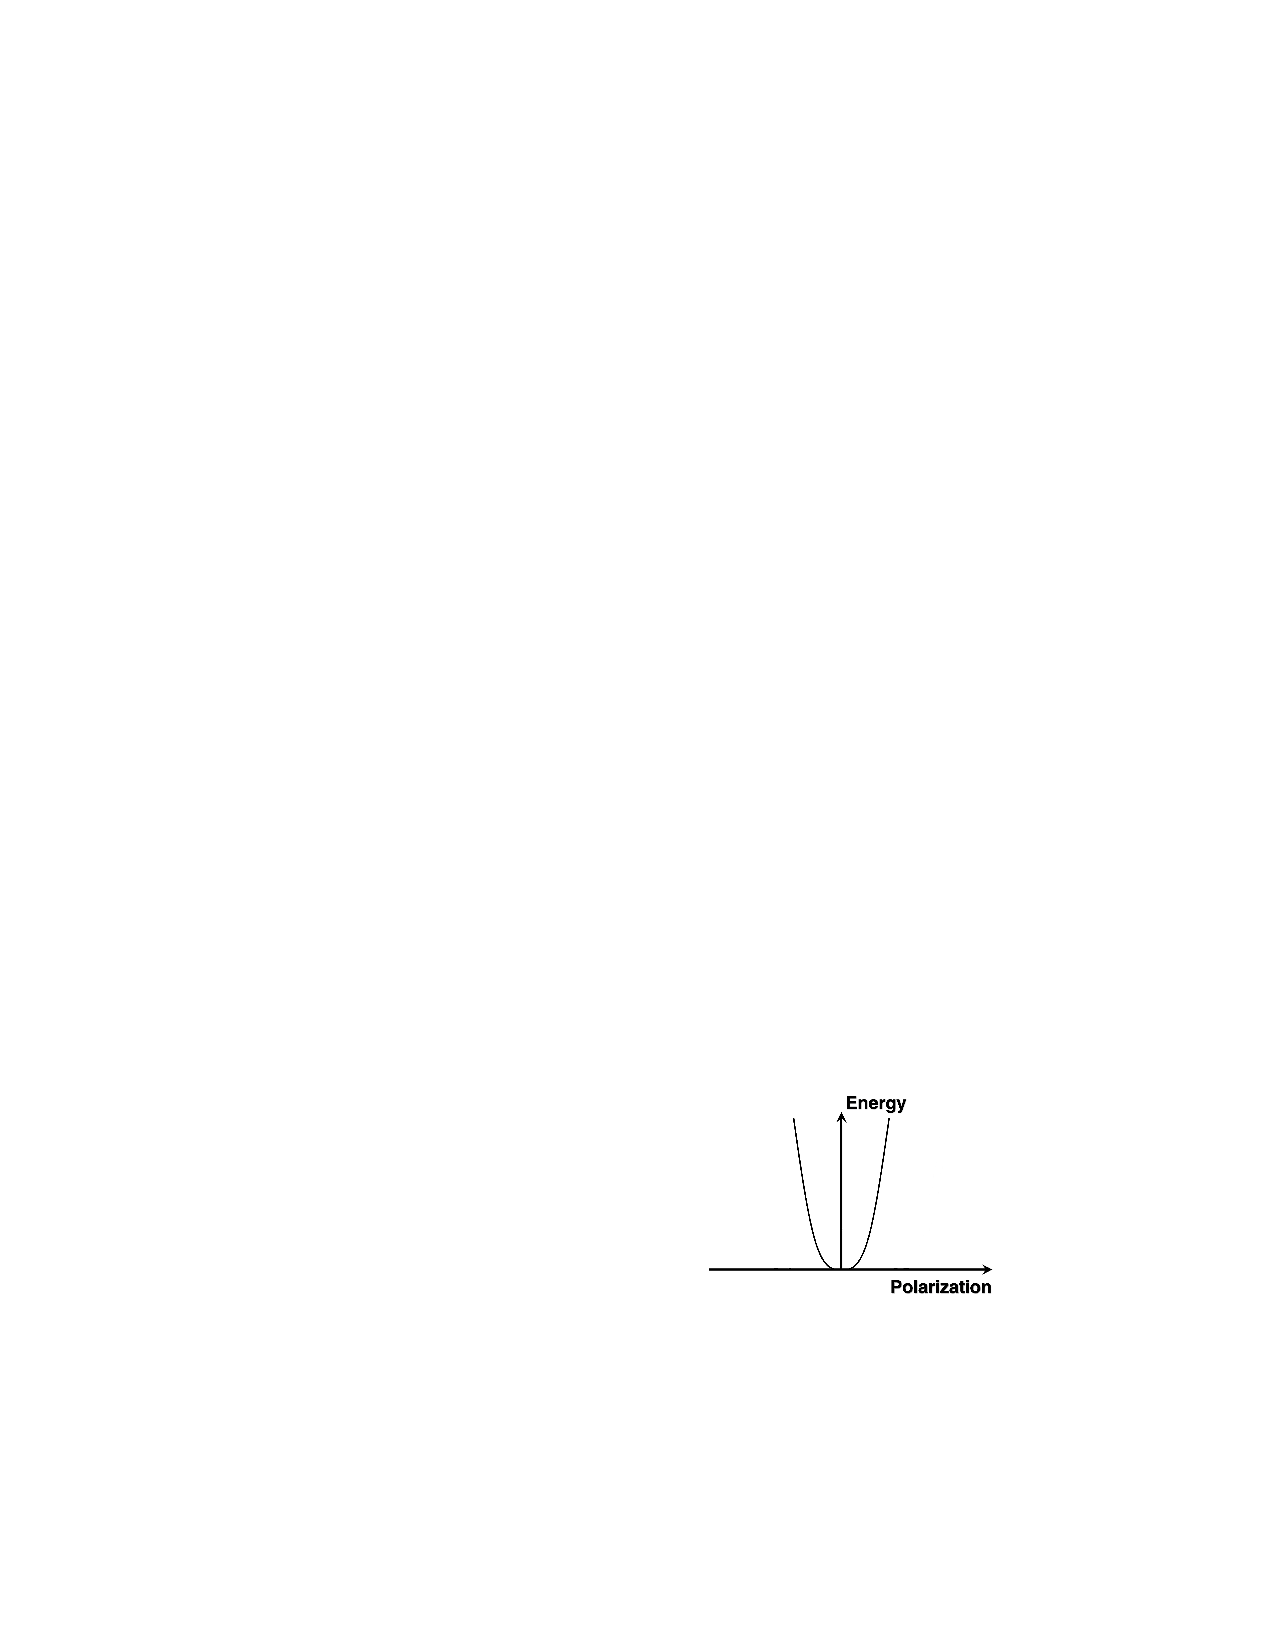
\includegraphics[width=0.45\linewidth]{./figures/materials/EvP-FE2}%
	} 	
   \subfloat[][Ferroelectric]{%
   	\label{fig:EvP-FE}%
	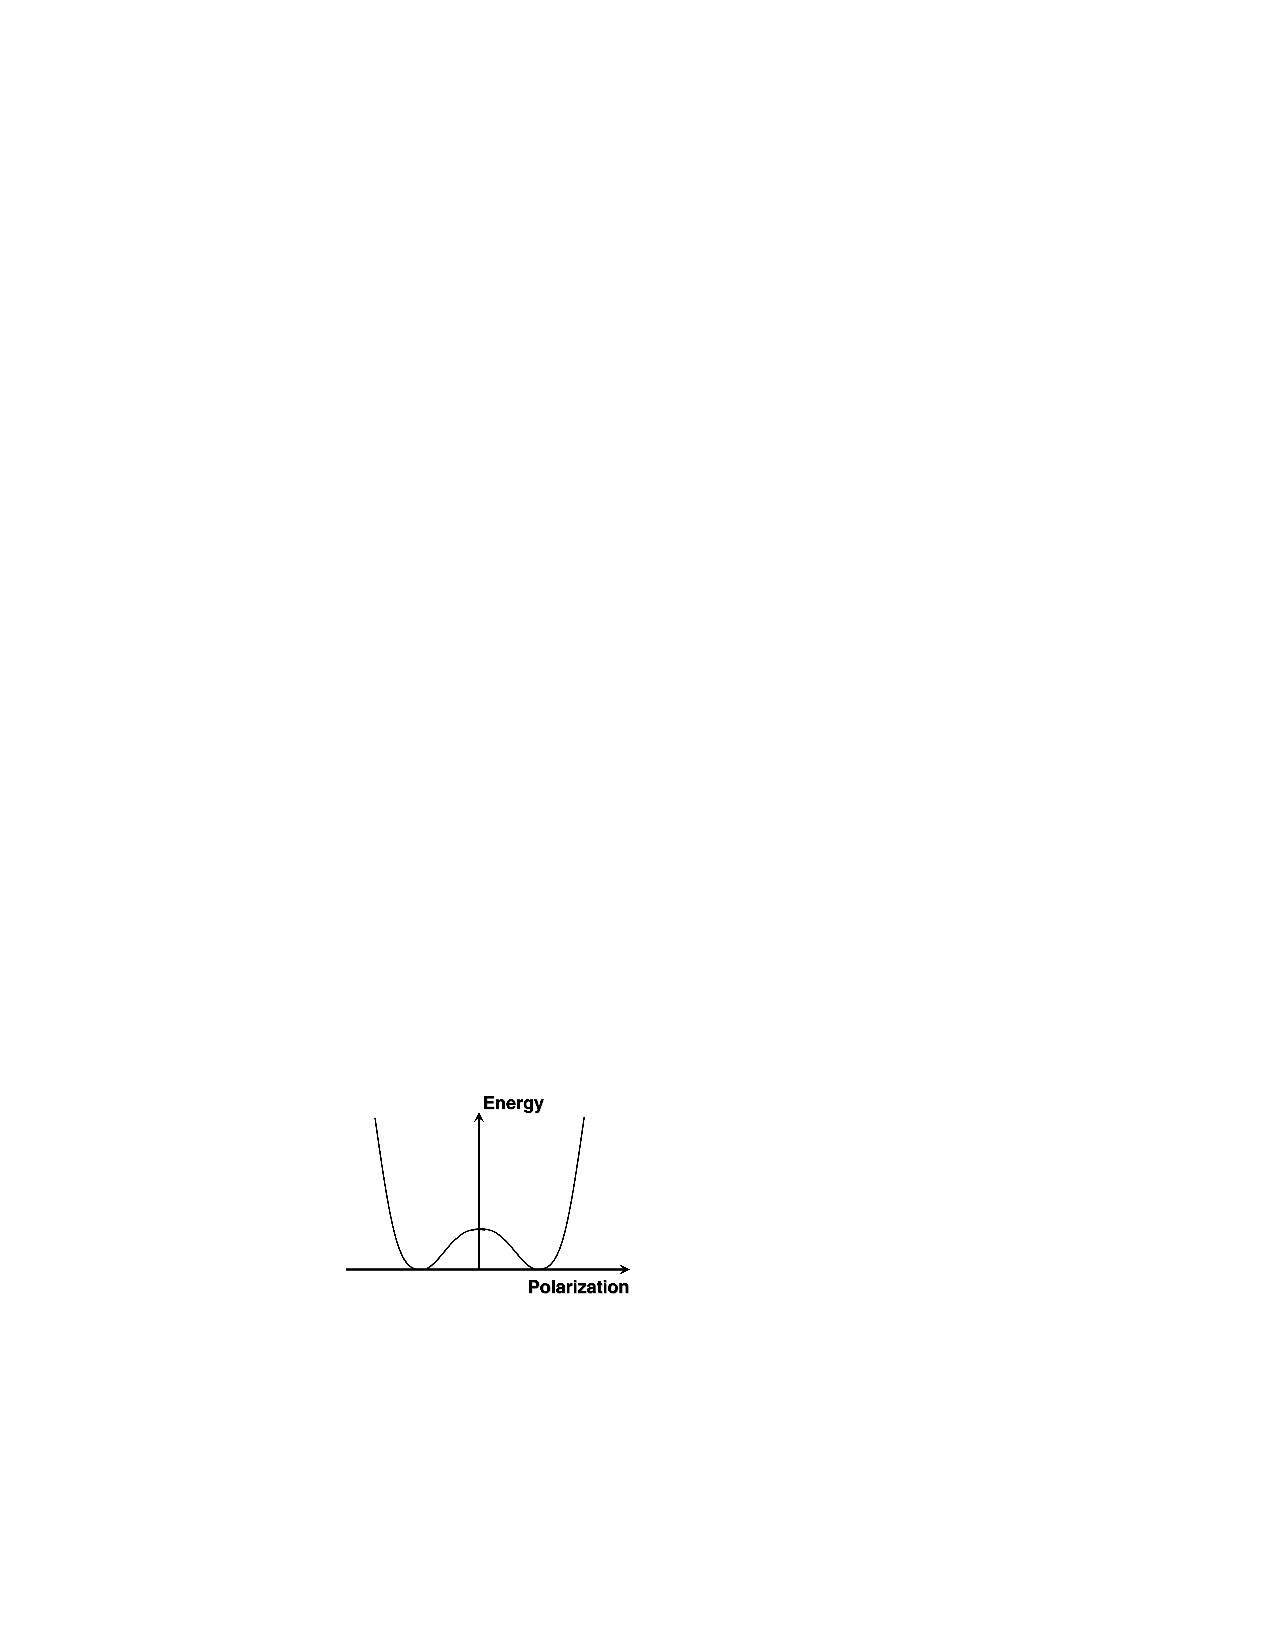
\includegraphics[width=0.45\linewidth]{./figures/materials/EvP-FE1}%
	} 	
   \caption[Energy vs. Polarization Plots for FE and PE Materials]%
   		{Example plots of the energy required to polarize a material. Ferroelectric materials (b) have %
		non-zero polarization at the energy minima. Above \Tc{} all ferroelectric materials transition %
		to a paraelectic phase (a). As temperature increases, the energy minima will approach one %
		another. These plots are generalized from equation~\vref{eq:landau-dev}.}
   \label{fig:EvP}
\end{figure}

\begin{figure}[tb]
   \centering
   \subfloat[][Paraelectric]{%
   	\label{fig:PvElec-PE}%
	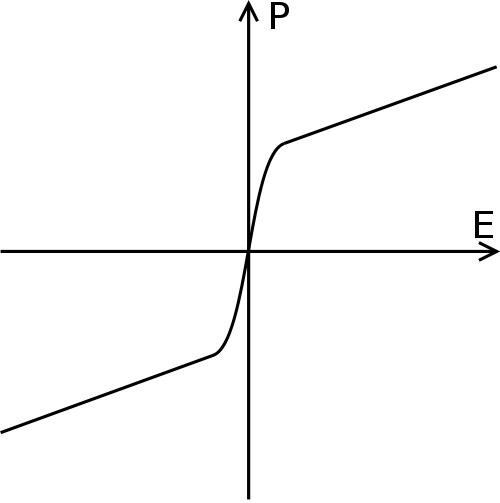
\includegraphics[width=0.4\linewidth]{./figures/materials/PvElec-PE}%
	} 
   \hspace{0.5cm}	
   \subfloat[][Ferroelectric]{%
   	\label{fig:PvElec-FE}%
	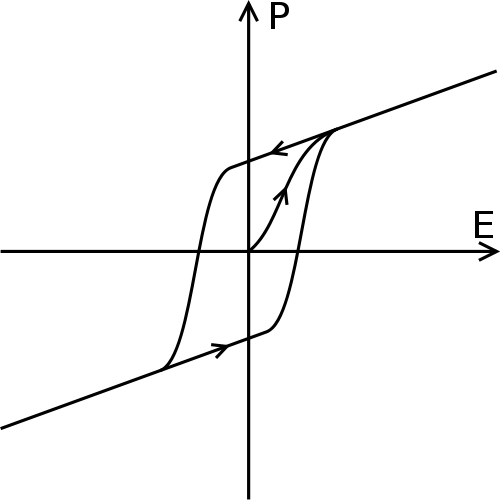
\includegraphics[width=0.4\linewidth]{./figures/materials/PvElec-FE}%
	} 	
   \caption[Polarization vs. Applied Field Plots for FE and PE Materials]%
   		{Example plots of the polarization as a function of applied field. (a) Paraelectric materials %
		have two regions of polarizability; at low E the polarization increases quickly with the field, %
		as E increases the rate of increase decreases. (b) Ferroelectric materials show similar %
		behavior, but additionally have hysteresis. This means that the films are switchable %
		between two states, but it is difficult to obtain zero polarization.\\%
		{\tiny Image Source: \url{http://en.wikipedia.org/wiki/Ferroelectricity} originally contributed by ``Bigly'' %
		under GNU-FDL.}}
   \label{fig:PvElec}
\end{figure}

%%%%%%%%%%%%%%%%%%%%%%%%%%%%%%%%%%%%%%%%%%%%%%%%%%%
%%%%%%%%%%%%%%%%%%%%%%%%%%%%%%%%%%%%%%%%%%%%%%%%%%%
%%%%%%%%%%%%%%%%%%%%%%%%%%%%%%%%%%%%%%%%%%%%%%%%%%%






























